\documentclass[a4paper,10pt]{article}
\usepackage[spanish]{babel}
\usepackage[utf8]{inputenc}
\usepackage{caratula}

\usepackage{amsmath}
\usepackage{amsfonts}
\usepackage[pdftex]{graphicx}
\usepackage{makeidx}
\usepackage{hyperref}
\usepackage{float}
\usepackage{caption}
\usepackage{subcaption}
\usepackage{color}
\usepackage{verbatim}
\usepackage{array}
\usepackage{tabularx}
\usepackage{multicol}
\usepackage{wrapfig}

\usepackage[top=3cm,bottom=2cm,left=2cm,right=2cm]{geometry}

\begin{document}

\materia{Aprendizaje Automático}

\titulo{Homework 4 : Supervised Learning}

\integrante{Martin Miguel}{181/09}{m2.march@gmail.com}

\maketitle
\tableofcontents
\newpage

\section{Introducción}

El presente trabajo presenta una comparativa entre 3 métodos de aprendizaje automático para estimar clasificadores. Se usaron tres aproximaciones distintas al problema de la clasificación: \emph{clasificación estadística} (en particular \textsf{naive bayes}), \emph{árboles de desición} y \emph{aprendizaje basado en instancias}. Para evaluar los métodos se realizaron \emph{cross-validation} con 10 folds sobre el dataset \textsf{adult}\footnote{\url{http://archive.ics.uci.edu/ml/datasets/Adult}}. Además, para hacer una comparación más completa, se ajustaron las configuraciones de los métodos para probar clasificadores más genéricos y más específicos, y todos estos se probaron sobre muestras de datos con variable ruido sobre el valor de la clase objetivo. 


\section{Ejecuciones}

\section{Resultados}

\begin{figure}
\centering
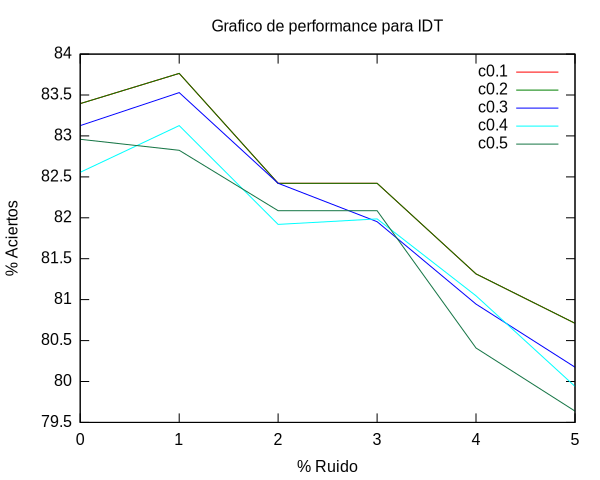
\includegraphics[width=\textwidth]{../dats/idt.pdf}
\caption{Gráfico de aciertos de los distintos clasificadores \textsf{IDT} con confianza variable sobre ruido variable.}
\end{figure}

\begin{figure}
\centering
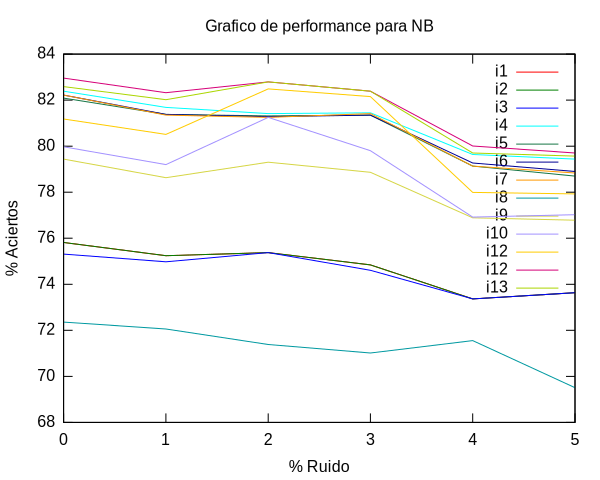
\includegraphics[width=\textwidth]{../dats/nb.pdf}
\caption{Gráfico de aciertos de los distintos clasificadores \textsf{NB} con atributos variables sobre ruido variable.}
\end{figure}

\begin{figure}
\centering
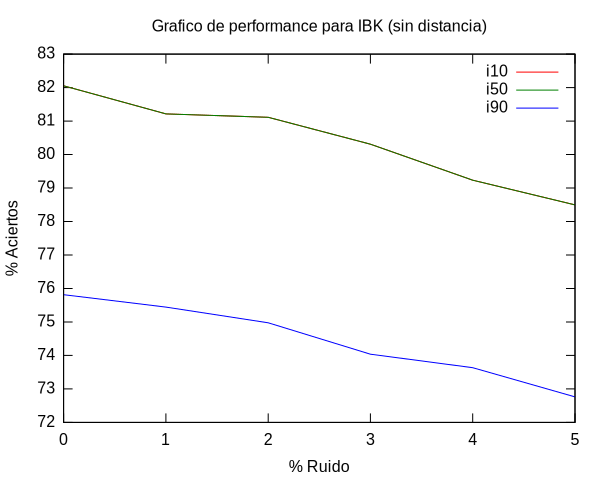
\includegraphics[width=\textwidth]{../dats/ibk-no.pdf}
\caption{Gráfico de aciertos de los distintos clasificadores \textsf{IBk} con cantidad variable de instancias sobre ruido variable, sin ponderar las instancias.}
\end{figure}

\begin{figure}
\centering
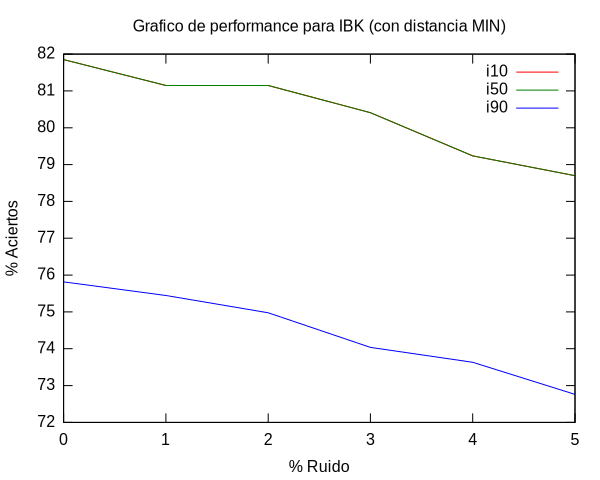
\includegraphics[width=\textwidth]{../dats/ibk-min.pdf}
\caption{Gráfico de aciertos de los distintos clasificadores \textsf{IBk} con cantidad variable de instancias sobre ruido variable, con ponderación $1-d$.}
\end{figure}

\begin{figure}
\centering
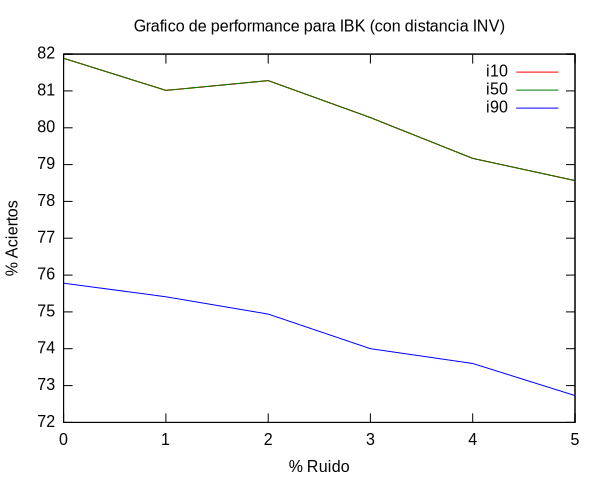
\includegraphics[width=\textwidth]{../dats/ibk-inv.pdf}
\caption{Gráfico de aciertos de los distintos clasificadores \textsf{IBk} con cantidad variable de instancias sobre ruido variable, con ponderación $1/d$.}
\end{figure}
\section{Conclusiones}



\end{document}

